\documentclass{article}

\usepackage{arxiv}
\usepackage[utf8]{inputenc} % allow utf-8 input
\usepackage[T1]{fontenc}    % use 8-bit T1 fonts
\usepackage{hyperref}       % hyperlinks
\usepackage{url}            % simple URL typesetting
\usepackage{booktabs}       % professional-quality tables
\usepackage{amsfonts}       % blackboard math symbols
\usepackage{nicefrac}       % compact symbols for 1/2, etc.
\usepackage{microtype}      % microtypography
\usepackage{amsmath}
\usepackage{lipsum}
\usepackage{caption}
\usepackage{float}
\usepackage{graphicx}
\usepackage{subcaption}

% the comment 'DATA POINT' will mark where data was calculated and then inserted into
% the paper.

\newcommand{\echonn}{\texttt{echonn}}
\newcommand{\der}[2][t]{\frac{\mathrm{d}#2}{\mathrm{d}#1}}

\title{Time Series Analysis of Chaotic Dynamical Systems with Recurrent Neural Networks}

\author{
  Lucas Wilson \\
  Undergraduate: Mathematics, Computer Science \\
  Colorado State University\\
  Fort Collins, CO 80523 \\
  \texttt{lkwilson96@gmail.com} \\
}

\begin{document}
\maketitle

\begin{abstract}
This is a paper about chaos.
\end{abstract}

%%% INTRODUCTION %%%
\section{Introduction}

Neural Networks are known to be able to approximate any function given enough
data and time to train \cite{cybenko1989approximation}. In light of this, the
hope is that a deep learning based model, the ESN, will outperform ARIMA.

This is a paper about chaos.
% TODO: Intro
% TODO: mention \texttt{echonn}

%%% CHAOS %%%
\section{Chaos}

%\subsection{History}

In 1963, Edward N. Lorenz published an article researching a simplified
system of ordinary differential equations modeling a convective system
\cite{lorenz1963deterministic}. His research popularized the possibility of a
system being highly sensitive to initial conditions, i.e., chaos theory;
while he wasn't the first to discover this phenomenon, he is considered to be
the "official discoverer of chaos theory" \cite{oestreicher2007history}.

When forecasting, the goal is to have accurate predictions. However, a
chaotic system's sensitivity to initial conditions implies that a small
perturbation as a result of error will produce incorrect solutions. Further,
given a periodic solution, the hope is that a small perturbation, from error
in measurement or from floating-point errors in numerical calculations,
doesn't affect the solution or at least produces a quasi-periodic solution
close to the periodic one. (A solution or trajectory $F$ is quasi-periodic if
and only if for all $t$ and for some $\tau$, $F(t+\tau)$ is arbitrarily close
to $F(t)$ \cite{lorenz1963deterministic}.)

An example of this is the trajectories of the sun and planets in our solar
system. Newton's equations can be used to create a system of equations to
model the bodies of mass (known as the n-body problem). However, with the
existence of other bodies of mass from other solar systems within the
universe, small perturbations are introduced into the system. If the system
is chaotic, then over time, the actual trajectories will diverge from our
model's \cite{oestreicher2007history}.
One of the defining characteristics of chaos is that the error from
perturbations grows exponentially \cite{oestreicher2007history}. At the time
of Lorenz's paper, unstable error was not well understood, and this led to
Lorenz's surprising discovery \cite{oestreicher2007history}. Lorenz reported
that a single iteration in calculating the solution to the dynamical system
took approximately one second \cite{lorenz1963deterministic}. In his paper,
he shows one of his calculations having about 3000 iterations, which must
have taken around 50 minutes. Given the amount of time it takes to perform
the calculation, it's tempting to continue the calculation from the output of
the previous calculation. However, the story of the discover is that while
the computer used 6 digit accuracy, it only output 3 digits, so when the
simulation was continued by Lorenz with the less accurate measurements, he
found the results to be very different \cite{oestreicher2007history}.

Chaos can appear in many different situations. Lorenz's paper demonstrates
chaos in a dynamical system useful for forecasting convection in the
atmosphere or liquids \cite{lorenz1963deterministic}. "Chaos theory has a few
applications for modeling endogenous biological rhythms such as heart rate,
brain functioning, and biological docks" \cite{oestreicher2007history}. It
can also appear in solutions to Hamiltonian problems such as the 3 body
problem (as mentioned before) and the double pendulum problem (as I will show
later). Understanding the predictability of chaos is very useful to many
different fields.

\subsection{Lyapunov Constant}

In terms of forecasting, it's useful to know how chaotic a dynamical system
is. Chaos will be measured by the exponential rate at which nearby
trajectories diverge. Constants describing the divergence are known as the
Lyapunov Characteristic Exponents (LCEs) \cite{sandri1996numerical}. There is
an LCE for each dimension, and since they all represent exponential growth.
The error growing at the rate of the largest LCE will dominate over the
others.

Given a small perturbation $\epsilon$ to a dynamical system in the direction
of the largest LCE, we can approximate the growth of the perturbation by the
equation $\epsilon(\Delta t) = \epsilon_0 e^{\lambda \Delta t}$ where
$\lambda$ is the largest LCE \cite{bezruchko2010extracting}. For an LCE of
zero, then the error doesn't grow exponentially, and thus, there is no chaos.
Error created from smaller LCEs is negligible. The approximate time scale
where perturbations become large is going to be proportional to $1 /
\lambda$. This is known as the Lyapunov time \cite{bezruchko2010extracting}.
For our solar system, the Lyapunov time is 10,000,000 years
\cite{oestreicher2007history}. Researchers have used it to evaluate the
effectiveness of forecasting models on chaotic problems
\cite{pathak2018model}. Predicting the solution of a chaotic model over an
interval of time which is multiple times the size of the Lyapunov time shows
the predictability of a model.

\subsection{Calculating the Largest Lyapunov Characteristic Exponent}
\label{sec:calc_lya}

In order to find the Lyapunov time, we only need to solve for the largest
LCE. To find this, we will use the following method detailed in
\cite{viswanath1998lyapunov}.

\newcommand{\xv}{\mathbf{x}}
\newcommand{\fv}{\mathbf{f}}
\newcommand{\Mv}{\mathbf{M}}

The dynamical system will be defined by $\der{\xv}=\fv(\xv)$ where $\fv, \xv
\in \mathbb{R}^d$. Given an initial condition $\xv_0$, the largest LCE,
denoted $\lambda_1$, is calculated as follows:

\begin{equation}
    \lambda_1 = \lim_{t \to \infty} \frac{1}{t}\log \sigma_1(\frac{\partial \xv(t)}{\partial \xv_0}) \label{eq:max_lce}
\end{equation}

where $\sigma_1$ is the first singular value of the matrix $\frac{\partial
\xv(t)}{\partial \xv_0}$ and $\log$ is the natural logarithm. Since we can
only numerically approximate the limit for $\lambda_1$, we will need to use a
sufficiently large $t$ until the limit converges to the accuracy we need.

In order to calculate $\frac{\partial \xv(t)}{\partial \xv_0}$, we need to
integrate the matrix differential equation:

\begin{equation}
    \der{\Mv(t)} = \frac{\partial \fv}{\partial \xv} \Mv(t)
    \label{eq:lce_mat_diffeq}
\end{equation}

where $\Mv(t) \in \mathbb{R}^{d \times d}$ and $\frac{\partial \fv}{\partial
\xv}$ is the $d \times d$ Jacobian matrix of $\fv(\xv)$ at $\xv(t)$.

Since values for $\xv(t)$ are needed as well, the systems will be integrated
together. If the dynamical system has dimensions $d$, then the new system of
differential equations will have dimension $d + d \times d$. For larger
dynamical systems, this calculation becomes costly. The dynamical systems
analyzed are small enough (having dimensions ranging from 3-4) that the
calculation can be performed timely and accurately.

There are several issues with calculating $\lambda_1$ with this algorithm.
Already mentioned, we need to choose a sufficiently large $t$ for the limit
to converge. Unfortunately, for chaotic systems, $\Mv$ will increase rapidly
with time. The large floating point values will eventually overflow and
$\lambda_1$ will not be accurate. I have found empirically that if values of
$\Mv$ don't exceed $10^{100}$, then $\lambda_1$ will be accurate.

Implemented in \echonn, the algorithm was tested on the Lorenz system for
various parameters and initial conditions. The LCEs match the expected values
very accurately (see the Lorenz System section: \ref{sec:lorenz}). The 3
dimensional 3-body problem is an 18 dimensional dynamical system, so while
the dynamical system is implemented in \echonn, its max LCE can't be
calculated accurately since the resultant system has 342 dimensions. The
algorithm was also tested on the differential equation which produces a
circle:

\begin{align*}
    x' &= y \\
    y' &= -x
\end{align*}

with the solution 

\begin{align*}
    x(t) &= r\sin(t) \\
    y(t) &= r\cos(t)
\end{align*}

for any $r \in \mathbb{R}$.

Given an initial condition $(x_0, y_0)$, it produces the trajectory of a
circle with radius $r=\sqrt{x_0^2 + y_0^2}$. If perturbed, the radius will
change, $r_\epsilon=\sqrt{(x_0+\epsilon_x)^2 + (y_0+\epsilon_y)^2}$, so the
new trajectory is

\begin{align*}
    x_\epsilon(t) &= r_\epsilon\sin(t) \\
    y_\epsilon(t) &= r_\epsilon\cos(t).
\end{align*}

Now, the $\ell^2$ norm of error is 
\begin{align*}
    \sqrt{(x_\epsilon - x)^2 + (y_\epsilon - y)^2} &= \sqrt{(r_\epsilon - r)^2\sin^2(t) + (r_\epsilon - r)^2\cos^2(t)} \\
    &= \sqrt{(r_\epsilon - r)^2(\sin^2(t) + \cos^2(t))^2} \\
    &= \sqrt{(r_\epsilon - r)^2} \\
    &= \vert r_\epsilon - r \vert.
\end{align*}

The error doesn't grow at all over time, so the LCE should be less than or
equal to zero as the system is not chaotic. The algorithm reports an LCE of
$-1.15954 \times 10^{-06}$ as expected.

Empirically shown, \echonn can be used to identify the max LCE of smaller
dynamical systems, and special precaution has to be taken when choosing a
time interval. Using a larger time will yield a more accurate $\lambda_1$,
but it may also cause an overflow if the system is chaotic. Thus, maximum
time values need to be chosen such that $\vert \vert \Mv\vert \vert_{\infty}$
doesn't exceed $10^{100}$ (where $\vert \vert \cdot \vert \vert_{\infty}$ is
the $\ell^\infty$ norm).

%%% DYNAMICAL SYSTEMS %%%
\section{Dynamical Systems}

Three dynamical systems will be used to demonstrate the predictability of
chaotic systems: the Lorenz system, Poincaré's 3-body problem solution, and
the double pendulum system. The Poincaré system is the one of the first, and
the Lorenz system is a classic example. The double pendulum is commonly
referred to as chaotic, and I will show this later. Both Poincaré's
restricted 3 body problem solution and the double pendulum are Hamiltonian
systems representing physical systems within our universe.

\subsection{Numerical Integration Methods}

In order to generate the data to be analyized, the solutions to these
dynamical systems need to be computed. Each of the systems are defined by a
system of differential equations which can be numerically solved. However,
due to the chaotic nature, error introduced by the numerical solution will
grow exponentially, so precaution need to be taken to avoid having this sort
of error introduced into the collected data. When numerically solving chaotic
problems, it's possible for the chaotic behavior to be suppressed, or where
there shouldn't be chaotic behavior, it could be created
\cite{corless1994good}.

However, it's been shown that the Fourth Order Runge-Kutta Method (RK4)
outperforms other numerical methods such as Euler's Method and the Midpoint
Method for chaotic systems \cite{zidan2011effect}. Not only does RK4 perform
better than other methods, it serves as a good method for producing accurate
numerical solutions to choatic systems with small enough time steps: the Lü
chaotic system \cite{mehdi2017using} and the Zhou system
\cite{roslan2013solving}, for example. One article points out that a larger
concern regarding these solutions is the accuracy of the initial conditions
measured from the physical problem which the mathematical model is based, but
otherwise, they echo the strength of correctly implemented numerical
solutions \cite{corless1994good}. Further, my initial conditions are randomly
generated, so this is not a concern.

I will be using an improved version of RK4 which incorporates the fifth order
Runge-Kutta: RK4(5) \cite{dormand1980family}. This is the method implemented
in the Python function \texttt{scipy.integrate.solve\_ivp}, and my numerical
solver wraps this function to integrate the chaotic systems. Using small time
steps will yield accurate samples from the chaotic systems.

\subsection{Lorenz System}
\label{sec:lorenz}

The Lorenz system was originally based on a system of equations modeling
convection created by Saltzman \cite{lorenz1963deterministic}
\cite{saltzman1962finite}. Simplified by Lorenz, it is defined as follows
\cite{lorenz1963deterministic}:

\begin{align}
    \der{x} &= \sigma (y - x), \nonumber \\
    \der{y} &= x (\rho - z) - y, \nonumber \\
    \der{z} &= x y - \beta z. \label{eq:lorenz_equation}
\end{align}

Not all parameters for the Lorenz equation will produce chaotic behavior. In
Lorenz's article, he uses the parameter values $\sigma=10$, $\beta=8/3$, and
$\rho=28$ \cite{lorenz1963deterministic}, and it has a maximum LCE of
$0.90566$ \cite{viswanath1998lyapunov}. There are other parameters which
produce chaotic results outlined in Table \ref{table:lorenz_params}. Also
shown in Table \ref{table:lorenz_params} are the values calculated by my
Python module \echonn are listed. These values are not as accurate, but
demonstrate the sufficient accuracy of \echonn.

\begin{table}[H]
    \centering
    \begin{tabular}{|l|l|l|l|l|l|l|}
        \hline
        $\sigma$ & $\rho$ & $\beta$ & actual $\lambda_1$ & calculated $\lambda_1$ & relative error of calculated $\lambda_1$ \\
        \hline \hline
        4 & 45.92 & 16 & 1.50255 & 1.49869 & -2.5694 $\times 10^{-3}$ \\ % DATA POINTS
        4 & 40 & 16 & 1.37446 & 1.37297 & -1.0876 $\times 10^{-3}$ \\
        8/3 & 28 & 10 & 0.90566 & 0.91188 & 6.8694 $\times 10^{-3}$ \\
        \hline
    \end{tabular}
    \caption{
        Lorenz Parameters and Largest Lyapunov Exponent
        \cite{viswanath1998lyapunov}
    }
    \label{table:lorenz_params}
\end{table}

The Lorenz system is named after its creator, but it is also known as the
Lorenz butterfly due to the shape of the system. The Lorenz Butterfly can be
seen in Figure \ref{fig:lorenz_butter}.

\begin{figure}[H]
    \centering
    \begin{subfigure}[b]{0.6\textwidth}
        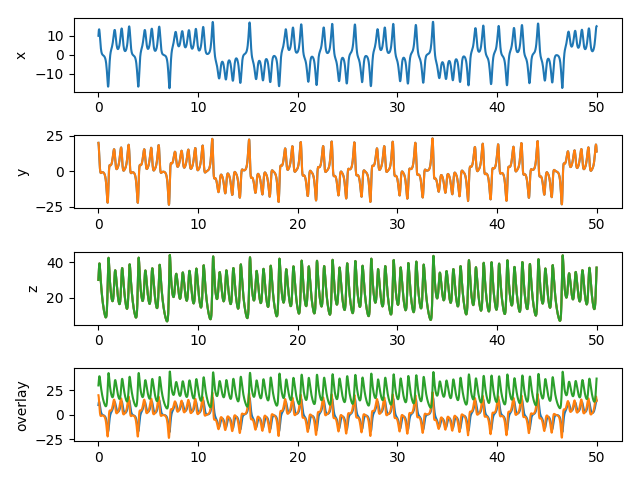
\includegraphics[width=\textwidth]{images/lorenz_nd_plot.png}
        \caption{Plot of each dimension of Lorenz System}
        \label{fig:lorenz_nd}
    \end{subfigure}
    \begin{subfigure}[b]{0.6\textwidth}
        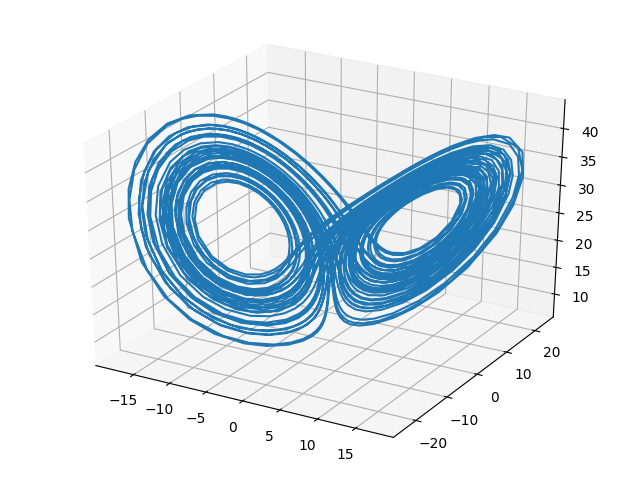
\includegraphics[width=\textwidth]{images/lorenz_3d_plot.png}
        \caption{The Lorenz Butterfly}
        \label{fig:lorenz_3d}
    \end{subfigure}
    \caption{The Lorenz System Visuals}
    \label{fig:lorenz_butter}
\end{figure}

\subsection{3-Body Problem}

The 3-body problem, or the generalized n-body problem, is a famous problem
which many have analyzed; most notably, Herni Poincaré wrote many papers
developing the area significantly \cite{chenciner2000remarkable}. One of
Poincaré's solutions, known as the circular restricted 3-body problem,
demonstrates chaotic properties \cite{oestreicher2007history}. Poincaré
performs several reductions of the original 3-body problem in order to come
to a much more useful form of the problem. The mass of one of the objects is
assumed to be negligible. This is the case for Sun-Earth-Moon orbits. The
moon has little effect on the orbit of the sun. Another aspect is the
rotating reference frame. Since the mass of one of the bodies is negligible,
the problem simplifies to first solving a two body problem. While much easier
to solver, Poincaré went further to stop the motion of the two planets by
using a rotating reference frame. Rotating with the planets, the problem can
be modeled seemingly by two static planets and a third mass-less planet
orbiting around those in a two dimensional plane.

% norm from https://tex.stackexchange.com/questions/107186/how-to-write-norm-which-adjusts-its-size
\newcommand{\norm}[1]{\left\lVert#1\right\rVert}
\newcommand{\rv}{\mathbf{r}}

The N body problem is defined as follows \cite{chenciner2000remarkable}:

Let $\rv_i$ be the position of the $i^\text{th}$ body in the N body problem.
Then, the force of gravity is the sum of gravity from every other body in the
system. That is,

\begin{equation}
   F_g^{(i)} = m_i \frac{\mathrm{d}^2 \rv_i}{\mathrm{dt}^2} =
   \sum_{j \neq i} G \frac{m_i m_j \hat{\rv}_{ij}}{\norm{\rv_{ij}}^3}
   \label{eq:nbody}
\end{equation}

where $\rv_{ij} = \rv_j - \rv_i$, $m_i$ is the mass of body $i$, and $G$ is
the gravitational constant.

For our purposes, the reduced system is more useful since it is much easier
to calculate than numerically solving the original 3-body problem. With three
bodies in three dimension, their motion is described by 9 second order
differential equations. Therefore, reducing the system to first order
differential equations yields 18 first order equations. The reduced problem
only requires 4 first order differential equations since the position is
defined by two second order differential equations.

Derived in two independent papers \cite{eberle2007case} and \cite{frnkacase},
the system of equations defined with dimensionless rotating (synodic)
coordinates:

\begin{align}
    x'' - 2 y' &= x
        - \frac{\alpha}{r_1^3} (x - \mu)
        - \frac{\mu}{r_2^3} (x + \alpha) \nonumber \\
    y'' + 2 x' &= \left(
        1 - \frac{\alpha}{r_1^3}
        - \frac{\mu}{r_2^3}
    \right) y \nonumber \\
\end{align}

where 

\begin{align}
    \mu &= \frac{m_1}{m_1 + m_2} \nonumber \\
    \alpha &= 1 - \mu \nonumber \\
    r_1(t) &= \left[(x(t) - \mu)^2 + y(t)^2\right]^{\frac{1}{2}} \nonumber \\
    r_2(t) &= \left[(x(t) + \alpha)^2 + y(t)^2\right]^{\frac{1}{2}} \label{eq:reduc_3body_cor}
\end{align}
 
and where mass body one and two are located at $-\alpha$ and $\mu$.

Although the notation in both papers was different, the equations were the
same. It's also worth mentioning that Eberle's paper was for his Masters
Thesis, and Frnka's paper has no details associated with it, but I was able
to find a mathematician with the exact name who achieved his doctorate. With
that said, I believe the math is reliable, and the simulations seem to work
and at least demonstrate chaotic properties (the only requirement for this
project). With my lacking physics knowledge, I was unable to derive these
equations myself from the assumptions made by Henri Poincaré outlined in
\cite{chenciner2000remarkable}.

If we define the following system:

\begin{align}
    x_1 &= x \nonumber \\
    x_2 &= x' \nonumber \\
    y_1 &= y \nonumber \\
    y_2 &= y', \label{eq:first_order_def}
\end{align}

then, we can take the derivative of each:

\begin{align*}
    x_1' &= x' \\
    &= x_2,
\end{align*}
and
\begin{align*}
    x_2' &= x'' \\
    &= 2 y' + x
        - \frac{\alpha}{r_1^3} (x - \mu)
        - \frac{\mu}{r_2^3} (x + \alpha) \\
    &= 2 y_2 + x_1 - \frac{\alpha}{r_1^3} (x_1 - \mu)
        - \frac{\mu}{r_2^3} (x_1 + \alpha),
\end{align*}
and
\begin{align*}
    y_1' &= y' \\
    &= y_2,
\end{align*}
and
\begin{align*}
    y_2' &= y'' \\
    &= - 2 x' + \left(
        1 - \frac{\alpha}{r_1^3}
        - \frac{\mu}{r_2^3}
    \right) y \\
    &= - 2 x_2 + \left(
        1 - \frac{\alpha}{r_1^3}
        - \frac{\mu}{r_2^3}
    \right) y_1.
\end{align*}

Then, we can represent the second order system of motion as four first order
equations:

\begin{align}
    x_1' &= x_2 \nonumber \\
    x_2' &= 2 y_2 + x_1 - \frac{\alpha}{r_1^3} (x_1 - \mu)
        - \frac{\mu}{r_2^3} (x_1 + \alpha) \nonumber \\
    y_1' &= y_2 \nonumber \\
    y_2' &= - 2 x_2 + \left(
        1 - \frac{\alpha}{r_1^3}
        - \frac{\mu}{r_2^3}
    \right) y_1, \label{eq:reduce_3_body_prog_sys} \\
\end{align}

where 

\begin{align}
    r_1 &= \left[(x_1 - \mu)^2 + y_1^2\right]^{\frac{1}{2}} \nonumber \\
    r_2 &= \left[(x_1 + \alpha)^2 + y_1^2\right]^{\frac{1}{2}}.
\end{align}

Here, $x_1$ and $y_1$ represent the position of the third body relative to
the other two, but not in the standard Cartesian coordinates of 3D space.
Outlined in the both papers, \cite{eberle2007case} and \cite{frnkacase}, the
transformation back to Cartesian coordinates is given, but we don't need the
exact position of the bodies since we are only concerned with the chaotic
motion, so that isn't shown here.

There are however two issues when integrating this problem. As objects
approach each other, the distance between them approaches zero. If collision
occurs, then this approaches infinity. There is no collision detection in
this model, and each body has a radius of zero, so this case is not handled.
Instead, a divide by zero error occurs, and the model cannot be calculated
further.

Further, near collisions are also an issue. With the distance between bodies
approaching zero, their potential energy becomes significantly smaller than
other values, such as those describing kinetic energy
\cite{chambers1999hybrid}. This produces a stiff system of equations, and
introduces error. Since energy is conserved in this Hamiltonian system, the
error introduced represents energy being created. This can cause the
singularity property seen in Figure \ref{fig:singularity}. This problem can
be solved by using a symplectic integrator \cite{chambers1999hybrid}.

\begin{figure}[H]
    \centering
    \begin{subfigure}[b]{0.4\textwidth}
        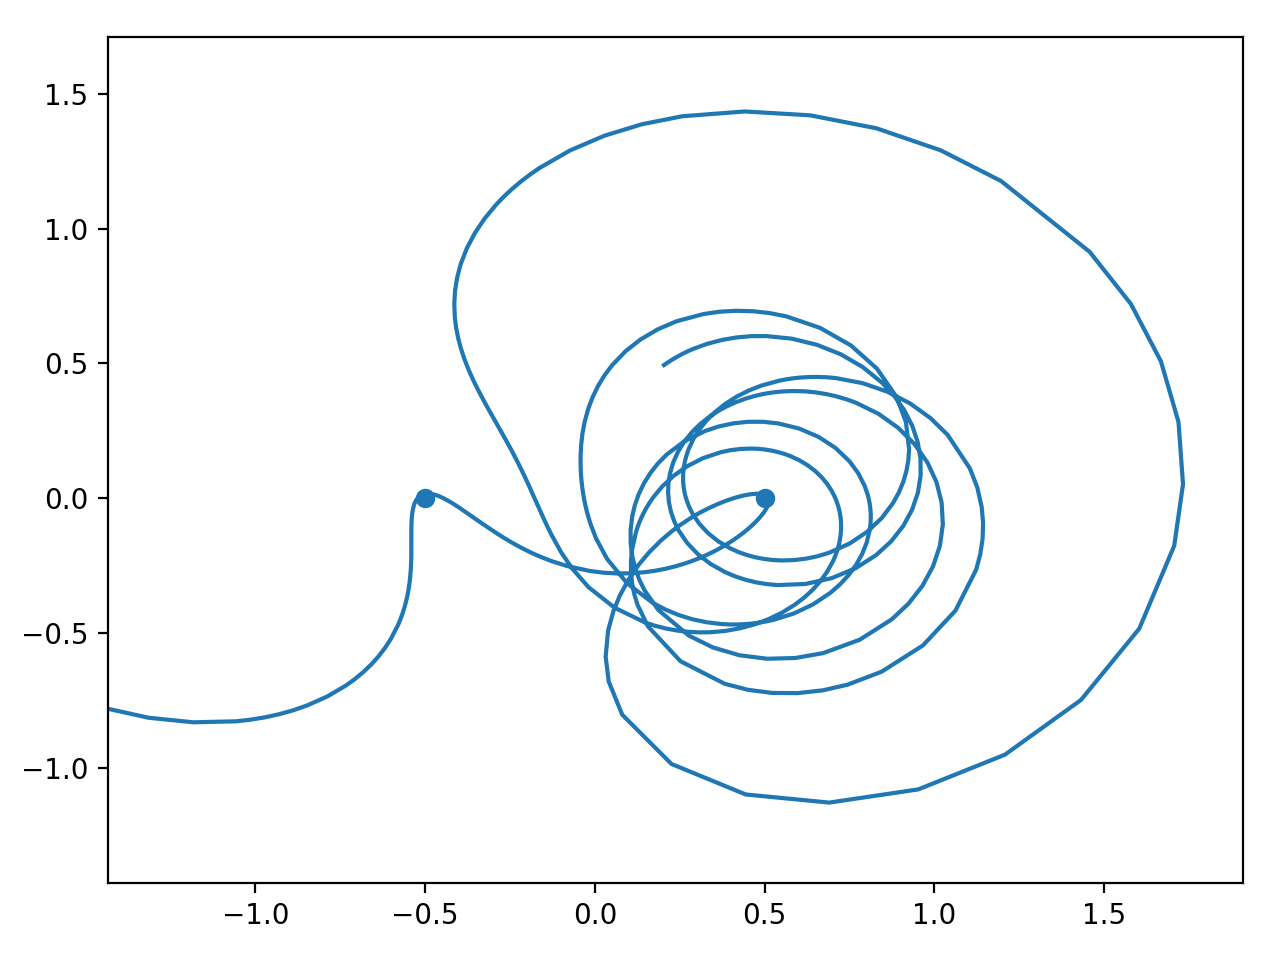
\includegraphics[width=\textwidth]{images/r3b_collision.png}
        \caption{Restricted 3 Body Problem with collision}
        \label{fig:r3b_collision}
    \end{subfigure}
    ~
    \begin{subfigure}[b]{0.4\textwidth}
        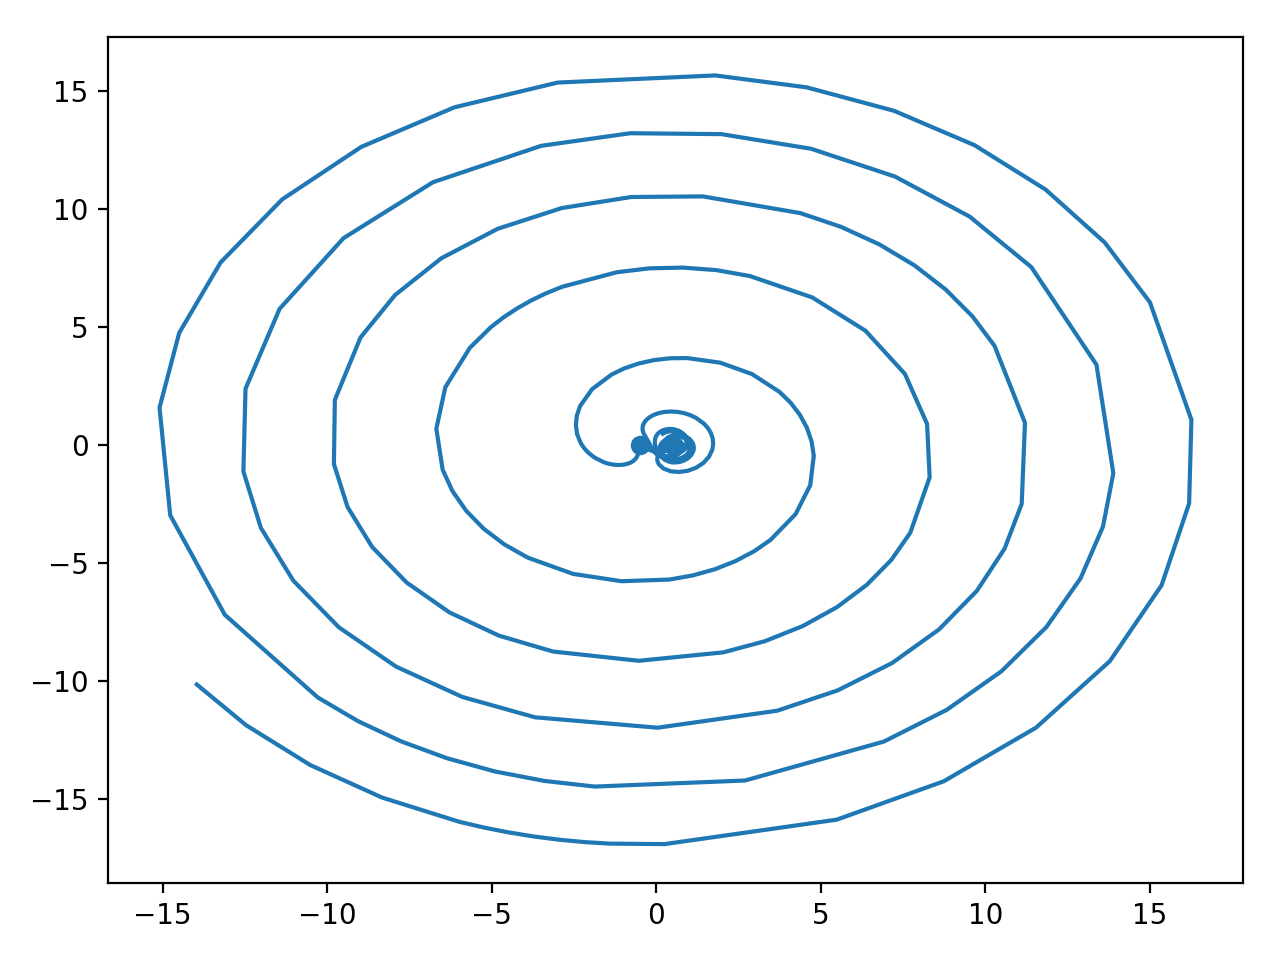
\includegraphics[width=\textwidth]{images/r3b_collision_whole.png}
        \caption{The resultant divergence of the body}
        \label{fig:r3b_collision_whole}
    \end{subfigure}
    \caption{The Restricted 3 Body Problem Error from Collision}
    \label{fig:singularity}
\end{figure}

While it is possible to use a symplectic integrator, it is not necessary.
Under the right initial conditions, the third body can diverge regardless
(fast initial velocity away from the bodies). The simple divergent spiral
isn't chaotic, so instead orbital and collision less initial conditions will
be used. Without divergence and without collisions, the symplectic integrator
is unnecessary.

\subsection{Double Pendulum}

The double pendulum is commonly cited to be chaotic
\cite{stachowiak2006numerical} \cite{levien1993double}. Using the system of
equations derived by Stachowiak \cite{stachowiak2006numerical}, the system is
defined as follows:

\begin{align}
    \der{\theta_1} &= \omega_1, \nonumber \\
    \der{\theta_2} &= \omega_2, \nonumber \\
    \der{\omega_1} &= 
    \frac{
        \sin(\theta_1 - \theta_2) \lbrack
            l_1 \cos(\theta_1 - \theta_2) \omega_1^2 + \omega_2^2
        \rbrack
    }{
        2 l_1 \lbrack
            1 + m_1 - \cos^2(\theta_1 - \theta_2)
        \rbrack
    }
    -
    \frac{
        (1 + 2 m_1) \sin \theta_1 + \sin(\theta_1 - 2 \theta_2)
    }{
        l_1 \lbrack
            1 + m_1 - \cos^2(\theta_1 - \theta_2)
        \rbrack
    }
    , \nonumber \\
    \der{\omega_2} &= \sin (\theta_1 - \theta_2) 
    \frac{
        (1+m_1) (\cos \theta_1 + l_1 \omega_1^2)
        +
        \cos(\theta_1 - \theta_2) \omega_2^2
    }{
        1 + m_1 - \cos^2(\theta_1 - \theta_2)
    }. \label{eq:doub_pen}
\end{align}

$\theta_1$ and $\omega_1$ represent the angle and angular velocity of the
inner pendulum where $\theta_1=0$ implies the pendulum is straight down, and
$\theta_1=\epsilon$ implies the pendulum is rotated $\epsilon$ radians
counter-clockwise. The same is true for the outer pendulum relative to its
pivot point, the end of the first pendulum. $l_1$ and $l_2$ are the lengths
of the inner and outer pendulums, respectively. $m_1$ and $m_2$ are the
masses of the balls on the end points of the inner and outer pendulums,
respectively. Then, the positions of the endpoints $(x_1$, $y_1)$ and $(x_2,
y_2)$ of the pendulum, with the center pivot at the origin, $(0, 0)$, can be
calculated as follows:

\begin{align}
    x_1 &= l_1 \sin(\theta_1), \nonumber \\
    y_1 &= - l_1 \cos(\theta_1), \nonumber \\
    x_2 &= x_1 + l_2 \sin(\theta_2), \nonumber \\
    y_2 &= y_1 - l_2 \cos(\theta_2), \label{eq:doub_pend_endpoints}
\end{align}

\begin{figure}[H]
    \centering
    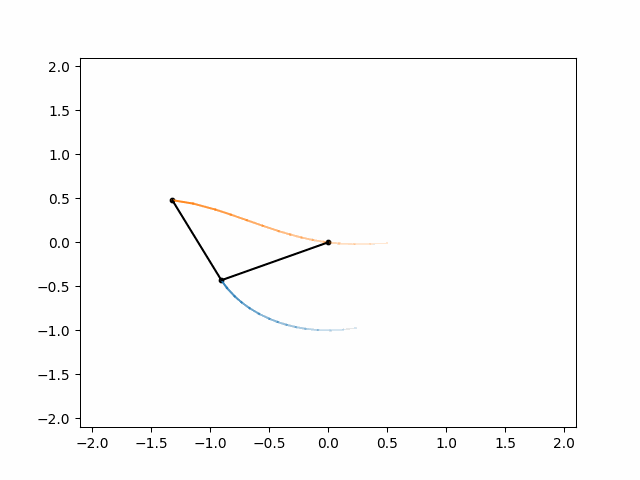
\includegraphics[width=.5\linewidth]{images/example_doub_pend.png}
    \caption{The Double Pendulum}
    \label{fig:doub_pend}
\end{figure}

While the system is a Hamiltonian system, Stachowiak decided to define the
first order derivative components as angular velocity as opposed to momentum.
This won't affect anything regarding the purpose of this paper.

Interestingly, the degree of chaos is dependent on the initial conditions
\cite{levien1993double}. In the experiment, the initial conditions had
angular velocities of zero, the outer pendulum was straight down, and the
inner pendulum varied from 0 degrees to 180 degrees \cite{levien1993double};
the results showed that the LCE increased with theta.

Repeating the same experiment, but with different parameters ($l_1 = l_2 =
1$, and $m_1 = m_2 = 1$), the results are similar (see Figure
\ref{fig:doub_pend_energy}). As inner theta increases, the largest LCE of the
system seems to approach 1.4. % DATA POINT

\begin{figure}[H]
    \centering
    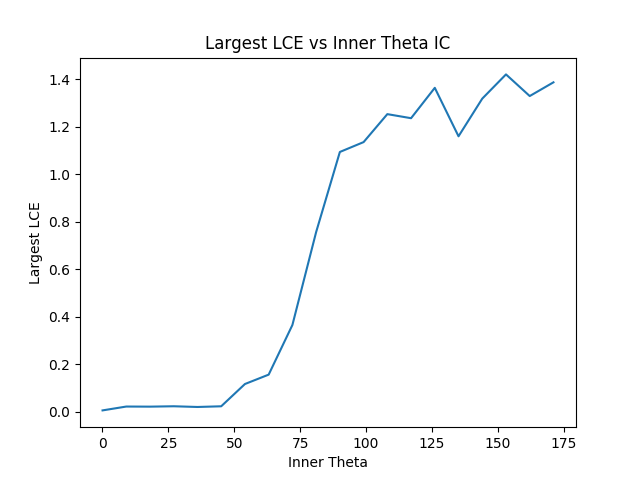
\includegraphics[width=.5\linewidth]{images/chaos_vs_energy_in_doub_pend.png}
    \caption{Largest Lyapunov Characteristic Exponent vs Inner Theta Initial Condition}
    \label{fig:doub_pend_energy}
\end{figure}

\section{The Echo State Network}

\newcommand{\Tv}{\mathbf{T}}
\newcommand{\Uv}{\mathbf{U}}
\newcommand{\Dv}{\mathbf{D}}
\newcommand{\tv}{\mathbf{t}}
\newcommand{\uv}{\mathbf{u}}
\newcommand{\dv}{\mathbf{d}}
\newcommand{\yv}{\mathbf{y}}
\newcommand{\Fv}{\mathbf{F}}
\newcommand{\wv}{\mathbf{w}}

The Echo State Network (ESN) is a type of Recurrent Neural Network (RNN) used
for time series analysis, but it is trained differently than most RNNs and is
characterized by having the echo state property. I implement the design
detailed by Jaeger in is 2002 book \cite{jaeger2002tutorial} and further
detailed in his 2007 article \cite{jaeger2007echo}.

A time series data set will contain samples of data which change over time.
Part of the data at each time point is measured or known before, called input
data and denoted by $\uv(t)$ with $K$ dimensions. The rest of the data will
be the goal for prediction, called output data and denoted $\dv(t)$ with $L$
dimensions.

For $T$ time samples, $t_1, t_2, \dots, t_T$, we have a $T \times K$ matrix,
$\Uv$, with sample input vectors as rows. We also have a $T \times L$ matrix,
$\Dv$, with sample output vectors as rows. A model will predict the values of
$\dv$, and this prediction will be denoted $\yv$.

\subsection{Recurrent Neural Networks and Traditional Training Method}
\label{sec:rnn}

RNNs are usually designed by having $K$ input units, $L$ output units, and
some internal units organized by some network structure. These units have
evolving values for every time point. The structure of networks describes how
units are connected. The input units at time $t_i$ are set to $\uv(t_i)$.
However, output units and internal units are calculated from the values of
other units. These other units are said to be connected to the resultant
unit. Output units are calculated from current input units, current internal
units, and from previous output units. Internal units are calculated from the
values of the current input units, previous internal units, and previous
output units.

Although, it's rare that the output units are calculated from previous output
units \cite{jaeger2002tutorial}. Sometimes for training, the output units are
set to the value of $dv$, called teacher forcing, so that the model trains on
actual values as opposed to its accumulated errors \cite{jaeger2002tutorial}.

To calculate the value of a unit, an activation function is applied to a
linear combination of the units connected to it
\cite{svozil1997introduction}. The constants for the linear combination are
called weights, and they are parameters of the model. Which activation
function is used is also a parameter of the function. Typically, some
non-linear function is used, such as $\tanh$, sigmoid, or rectified linear
unit.

During training, we search for weights which maximize the model's performance
on data which the model hasn't seen. A common training method for RNNs is to
use a form of backpropagation \cite{jaeger2002tutorial}. Backpropagation for
RNNs is slightly different from traditional Neural Networks, but the idea is
the same.

For example, given some neural network model $\yv(\xv; \wv)$, where $\xv$ is
known input data, $\wv$ is the model's parameters, and $\yv$ approximates
some values, $\tv$, then we define an objective function as the sum of
squared error:

\newcommand{\Ev}{\mathbf{E}}

\begin{equation}
    \Ev(\xv; \wv) = \vert \vert \yv(\xv; \wv) - \tv \vert \vert_2^2.
    \label{eq:error_eq_rnn}
\end{equation}

Using steepest descent to solve this minimization problem (as shown in
\cite{svozil1997introduction}), we can reduce $\Ev$ in
(\ref{eq:error_eq_rnn}) by updating the weights as follows:

\begin{equation}
    \wv = \wv - \lambda \nabla_\wv \Ev
\end{equation}

for some learning rate $\lambda$.

\subsection{Echo State Network Implementation}

The implementation design used for this paper is detailed by Herbert Jaeger
in \cite{jaeger2002tutorial} and \cite{jaeger2007echo}. I explain it here to
clarify my exact process (and with a slight change of notation to be
consistent with the rest of this paper).

Like RNNs, ESNs have an input layer with $K$ units and with values $\uv(t_1),
\uv(t_2), \dots, \uv(t_T)$ where $\uv(t) \in \mathbb{R}^K$. $K$ is zero if
there are no input units. There is an internal layer with $N$ units, denoted
by $\xv(t_i) \in \mathbb{R}^N$ for $i = 1, 2, \dots, T$, and there is an
output layer with $L$ units, denoted by $\yv(t_i) \in \mathbb{R}^L$ for all
$i = 1, 2, \dots, T$.

\newcommand{\W}{\mathbf{W}}
\newcommand{\Win}{\mathbf{W}_{in}}
\newcommand{\Wback}{\mathbf{W}_{back}}
\newcommand{\Wout}{\mathbf{W}_{out}}

How the units are connected can vary, but the suggested way
\cite{jaeger2002tutorial} is to connect the internal layer to the current
input layer, the previous internal layer, and the previous output layer.
These connections will have weights described in \ref{sec:rnn}. Respectively,
these weights will be denoted by the matrices: $\Win$, $\W$, and $\Wback$.
The activation function for the internal layer is $\tanh$.

The output layer is connected to the current input layer and current internal
layer. Additionally, a bias input is connected to this layer. The weight for
these connections will be denoted $\Wout$ (we only have one matrix since the
connected layers are concatenated into a single vector, per Jaeger's notation
\cite{jaeger2002tutorial}). The activation function for these connections is
linear. Although, the recommended choice is $\tanh$, the output layer doesn't
necessarily lie in the range of $\tanh$, so it can't be used without some
form of normalization.

In mathematical notation, the model is defined as follows:

\begin{align}
    \xv(t_{i}) &= \tanh \left(
            \Win \uv(t_i)
            + \W \xv(t_{i-1})
            + \Wback \yv(t_{i-1})
        \right) \\
    \yv(t_i) &= \Wout (\uv(t_i), 1, \xv(t_i))_{\text{concat}}.
\end{align}

$\xv$ and $\yv$ are calculated from previous unit values but for the first
time step, there are none, so we need to initialize the units to zeros
\cite{jaeger2002tutorial}. This is done by defining $\xv(t_0)$ and $\yv(t_0)$
to zeros.

The weights are initialized such that the model has the defining
characteristic of echo state networks: the echo state property (Section
\ref{sec:eprop}). During the training phase (Section \ref{sec:etrain}),
$\Wout$ is fit to the training data.

Once the network has been initialized and trained, it can be used to perform
time series analysis.

\subsection{The Echo State Property}
\label{sec:eprop}

The echo state property is defined by the following
\cite{jaeger2002tutorial}:

\begin{quote}
    Assume an untrained network with weights $\Win$, $\W$, and $\Wback$ is
    driven by teacher input $\uv(n)$ and teacher-forced by teacher output
    $\dv(n)$ from compact intervals $\Uv$ and $\Dv$. The network ($\Win$,
    $\W$, and $\Wback$) has echo states w.r.t. $\Uv$ and $\Dv$, if for every
    left-infinite input/output sequence $(\uv(n), \dv(n-1))$, where $n=\dots,
    -2, -1, 0$, and for all state sequences $\xv(n)$, $\xv'(n)$ compatible
    with the teacher sequence, i.e. with
    \begin{align}
        \xv(n) &= \tanh \left(
                \Win \uv(n)
                + \W \xv(n-1)
                + \Wback \yv(n-1)
            \right) \\
        \xv'(n) &= \tanh \left(
                \Win \uv(n)
                + \W \xv'(n-1)
                + \Wback \yv(n-1)
            \right)
    \end{align}
    it holds that $\xv(n) = \xv'(n)$ for all $n \leq 0$.
\end{quote}

The idea is that if the network is run long enough, it will, in a sense,
forget long past input and focus only on the most recent input. If two
networks with differing internal states are run with the same input and
teacher-forced output, they will eventually converge to each other. It's name
suggests data fed to the model will echo around but eventually fade as echos
do.

Jaeger outlines a process to create weights which will likely have echo state
properties. The process is posed as conjecture and doesn't guarantee the echo
state property. However, the echo state is very likely and can be assumed
confidently \cite{jaeger2002tutorial} \cite{jaeger2007echo}.

To demonstrate the echo state property, initialize the network with random
values. Set user input (if any) and teacher-forced output units to zero,
After enough iterations, the internal state should converge to zero.

The process to initialize the echo state weights, $\W$, is as follows
\cite{jaeger2002tutorial}:

\newcommand{\specrad}{\vert \lambda_\text{max} \vert}
\begin{enumerate}
    \item Initialize an $N \times N$ matrix, $\W_0$, with values from a 
    uniform distribution in $[-1, 1]$.
    \item Calculate the spectral radius, $\specrad$, of $\W_0$, i.e., the 
    maximum absolute value of the eigenvalues of $\W_0$.
    \item Normalize $\W_0$ to $\W_1$ so that it has unit spectral radius:
    $\W_1 = \frac{1}{\specrad} \W_0$
    \item Choose parameter $\alpha < 1$. Typically, $\alpha$ lies in
    the range $(0.7, 0.98)$ \cite{jaeger2002tutorial}. This number will 
    represent the new spectral radius of $\W$.
    \item Scale $\W_1$ to $\W_2$ to have a spectral radius of
    $\alpha$: $\W_2 = \alpha \W_1$. Now, let $\W = \W_2$, and the model
    will have the echo state property \cite{jaeger2002tutorial}.
\end{enumerate}

If the spectral radius of $\W$ is found to be greater than 1, then it can be
shown that the model doesn't demonstrate the echo state property; Jaeger's
process uses this fact by ensuring that this isn't the case
\cite{jaeger2002tutorial}. While it can't guarantee an echo state property,
the resultant matrix does have the property frequently enough that it's a
reliable process. In his words, the model "has always been found to be an
echo state network" \cite{jaeger2002tutorial}.

\newcommand{\vv}{\mathbf{v}}

Applying linear algebra, this makes a lot of sense. Let $A$ be an $N \times
N$ matrix with spectral radius $r = \rho(A) > 0$ and denote its eigenvalues
$\lambda_i$ and eigenvectors $\vv_i$ for $i = 1, 2, \dots, N$. Then, define
$B = \frac{\alpha}{r} A$.

By definition, $\vv_i A = \lambda_i \vv_i$, so
\begin{align*}
   \vv_i B &= \frac{\alpha}{r} \vv_i A \\
   &= \frac{\alpha}{r} \lambda_i \vv_i
\end{align*}

Therefore, $B$ has eigenvalues $\frac{\alpha}{r} \lambda_i$ for all $i$.
Further, its spectral radius is then

\begin{align*}
    \vert\vert \frac{\alpha}{r} \lambda \vert\vert_\infty
    &= \frac{\alpha}{r} \vert\vert \lambda \vert\vert_\infty \\
    &= \frac{\alpha}{r} r \\
    &= \alpha
\end{align*}

where $\lambda$ is a vector of eigvenvalues and $\vert \vert \cdot \vert
\vert_\text{max}$ is the $\ell^\infty$ norm.

As the model iterates, the matrix transformation of $B$ is repeatedly
applied. With $\uv$ and teacher-forced $\dv$ as zeros, the internal state has
the value $\xv(t_{k+1}) = \tanh(B \xv_k)$ for iteration $k$.

Since the spectral radius of $B$ is less than 1,
\begin{align*}
    \lim_{k \to \infty}B^k \vv_i &= \lim_{k \to \infty} \lambda_i^k \vv_i & \text{ (where $\lambda_i$ and $\vv_i$ is an eigvenvalue-eigenvector pair of $B$)} \\
    &= 0 \vv_i & \text{ (since $\vert\lambda_i\vert < \alpha < 1$ and $\lim_{k \to \infty}\alpha^k = 0$)} \\
    &= 0
\end{align*}

This suggests that as the model iterates, the internal state converges to
zero.

The rest of weights can be initialized however desired, so we will use a
common technique.

\begin{enumerate}
    \item Initialize an $N \times M$ matrix, $\W_0$, with values from a 
    uniform distribution in $[-1, 1]$. $M$ and $N$ here are not the 
    same values from before for the sake for generality. 
    \item Scale the matrix by $\frac{1}{\sqrt{M}}$ to calculate the weight matrix.
\end{enumerate}

Then, $\Win$ and $\Wback$ can be calculated as follows:

\begin{align}
    \Win &= \frac{\W_0}{\sqrt{K}} \nonumber \\
    \Wback &= \frac{\W_0}{\sqrt{L}} \nonumber
\end{align}

Different from most training techniques, $\Win$, $\W$, and $\Wback$ are never
changed after initialization.

\subsection{Echo State Network Training}
\label{sec:etrain}

In order to train the echo state network, we need to find good weight values
for $\Wout$. Training the echo state network is different from the
backpropagation approach in that we can solve for and calculate directly the
weights matrix; more modern methods use an iterative approach which converges
to good weight values. Part of the reason is due to the calculation cost of
the iterative methods. Today, that it is no longer an issue, but
historically, it was a strong quality of the echo state network
\cite{jaeger2007echo}.

First, the data (input, $\uv$, and output, $\dv$, values) is partitioned into
three groups:
\begin{enumerate}
    \item Initialization values at time points
    $t_0, t_1, \dots, t_{T_0-1}$.
    \item Training values from
    $t_{T_0}, \dots, t_T$
    \item Testing values from
    $t_{T+1}, \dots, t_{T_f}$
\end{enumerate}

Second, the initialization data is fed into the model. This initializes the
inner state of the model, and the initial state (zeros) is lost due to the
echo state property. $T_0$ should be chosen such that this is truly the case.
Like $\alpha$, $T_0$ is a parameter of the echo state network and differs
depending on the problem. Good values for $T_0$ are 10 to 500 depending on
the problem complexity.

Third, the training values are fed into the model to sample the network. We
can store the input unit values, the internal state values, and the desired
output values as matrices $M$ and $T$. $M$ will store the input unit values
and internal state value pairs $(\uv(t_{T_0}), 1, \xv(t_{T_0})), \dots,
(\uv(t_T), 1, \xv(t_T))$ in its rows. $T$ will store the output unit values
$\dv(t_{T_0}), \dots, \dv(t_T)$.

To train the model, we want $\Wout M$ to approximate accurately $g^{-1}(T)$,
where $g$ is the activation function for the output layer. Since we use an
idempotent output layer activation function, $g^{-1}(T) = T$.

Therefore, $\Wout$ should be found such that $\Wout M = T$
\cite{jaeger2002tutorial}. Solving for $\Wout$,

\begin{align*}
    \Wout M &= T \\
    (\Wout M)^T &= T^T & \text{ (where $A^T$ is the transpose of $A$)} \\
    M^T \Wout^T &= T^T \\
    (M^T)^{-1} M^T \Wout^T &= (M^T)^{-1} T^T & \text{ (where $A^{-1}$ is the Moore-Penrose pseudoinverse \cite{ben2003generalized} of $A$)} \\
    \Wout^T &= (M^T)^{-1} T^T \\
    \Wout &= \left((M^T)^{-1} T^T\right)^T \\
    \Wout &= T \left((M^T)^{-1}\right)^T
\end{align*}

Using packages like \texttt{numpy.linalg.eig} and \texttt{numpy.linalg.pinv},
solving for eigenvalues and pseudoinverses for $\Wout$ is very easy. After
solving for $\Wout$, the echo state network is trained.

To evaluate the network, the testing values are fed into the model. However,
this time, the output layer is not teacher-forced since in real application,
the output values are unknown. To measure how well the echo state network
approximates the desired output we define the error to be the root mean
squared error (RMSE) of the actual output values $\dv$ and predicted values
$\yv$: $\sqrt{\sum_{i=T+1}^{n} (\dv(t_i) - \yv(t_i))^2}$ where $n \in [T+1
\dots T_f]$. The error represents the predictive power of the model for $n$
time steps in the future. If RMSE is low for larger values of $n$, the model
has a strong long term predictive power.

%noise: 0.0001 to 0.01 \cite{jaeger2002tutorial}

%\subsection{LTSM}

%%% ANALYSIS %%%
\section{Analysis}

\subsection{Method}

First, data from the models is collected. Using the process described above
(Section \ref{sec:calc_lya}), the Largest Lyapunov Exponent is calculated,
$\lambda_1$. Then, the Lyapunov Time is calculated by $\frac{1}{\lambda_1}$.
We will then integrate the model with an algorithm called RK4(5) over the
interval $[0, \frac{50}{\lambda_1}]$ with time steps of $\frac{1}{100
\lambda_1}$. This will result in 5,000 data points.

Then, the data is partitioned into a training set, a validation set, and a
testing set. I use a 90\% split, so testing is the last 10\% of the data. The
training and validation set are the first 90\%. Of the 90\%, training is the
first 90\%, and validation is the final 10\%. In total, it's a 81\%-9\%-10\%
split.

The training set is used to train the model. The validation set is used to
tune the parameters of the model ($\alpha, N, T_0$). The testing set is used
to evaluate the performance.

The first data point of the training set is $t_0 = 0$. The parameter $T_0$
marks where the model begins training on the data (see Section
\ref{sec:etrain}). Using slightly different notation to account for the extra
validation set, we will denote the first validation time point by $t = T$. We
will denote the first testing time point by $t = T_f$

Performance of the model is calculated by RMSE for a given time interval
$[t_0, t_f]$:

\begin{align}
    \text{RMSE} = \sqrt{\sum^{t_f}_{t=t_0} (\dv(t) - \yv(t))^2}
\end{align}

where $(\cdot)^2$ is the dot product of the error with itself, $\dv(t)$ is
the true value at time $t$, and $\yv(t)$ is the model's approximation at time
$t$.

First, we generate a list of parameter combinations to try. Usually, this is
the Cartesian product of typical parameter values for the model. For each
combination, we train several models on the training data. Then, we predict
the validation data to measure the general performance of the model under
those parameters.

$\text{RMSE}_\text{train}$ is calculated on the interval $[T_0, T)$, and the
prediction uses teacher-forced values on $[0, T_0)$.
$\text{RMSE}_\text{validation}$ is calculated on the interval $[T, T_f)$, and
the prediction uses teacher-forced values on $[0, T)$.

Then, the models which performed best on the validation set should also
perform well on the testing set. The models are retrained on the testing and
validation set, and the error is calculated: $\text{RMSE}_\text{full train}$
is calculated on the interval $[T, T_f)$, and the prediction uses
teacher-forced values on $[0, T)$.

Finally, the error for the testing set is calculated. The performance on the
testing set is an unbias representation of how well the ESN can fit the
model.

However, the $\text{RMSE}_\text{test}$ is calculated slightly different since
we want to know how far the model can predict before deviating too far. The
$\text{RMSE}_\text{test}(t_f)$ will be calculated on the interval $[T_f,
t_f)$ and the prediction uses teacher-forced values on $[0, T_f)$. Lastly,
$\text{RMSE}_\text{test}$ will notate the RMSE for the entire test set.

We will look at how far past $T_f$ the ESN model's $\text{RMSE}_\text{test}$
grows too large. The best model will be the model with the lowest Testing
RMSE for the longest time.

\subsection{Results}
\subsubsection{Lorenz}

To integrate the model, I use the initial conditions: $(x_0, y_0, z_0) =
(-13.78990503, -11.6069343, 36.17332518)$. The calculated Lyapunov value was
$0.9348566$.

One of the issues run into while forecasting with the Lorenz is that the
continuous nature of the equation led to the ESN just outputing the previous
value. For initial values far from the center of the Lorenz Butterfly, it
would tend towards the center and stop when it does arrive there. Most models
trained poorly and gave $\text{RMSE}_\text{test}$ values of 16 or well above
10,000, implying the model diverged.

To fix this issue, we instead have the ESN train on differences between time
points. This reduces our data set to 4,999 values, and it creates a new shape
of the data. The Lorenz Butterfly had a similar shape, two rings, but in this
case, the rings intersect (See figure \ref{fig:lorenz_diff}).

\begin{figure}[H]
    \centering
    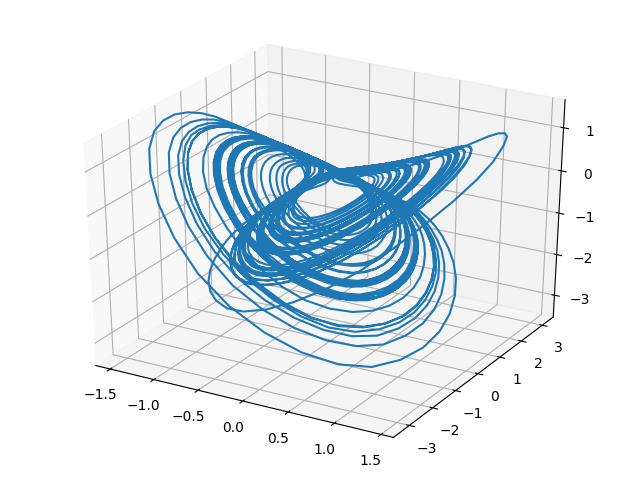
\includegraphics[width=.5\linewidth]{doc/paper/images/lorenz/full_differential.png}
    \caption{A plot of the differences between time steps of an approximation of the Lorenz Butterfly}
    \label{fig:lorenz_diff}
\end{figure}

After this transformation of the data, the model performed significantly
better. $\text{RMSE}_\text{test}$ dropped to ranges of 1-2, the model
exploded (diverged to infinity) less frequently, and it was no longer
outputting previous values.

Most well performing models couldn't predict past one Lyapunov constant. From
the graphs, we can see that most models deviated once reaching the
intersection of the butterfly wings.

Once reaching the intersection, several things can happen. First, it can
deviate completely and stop following either wings. Second, it can follow the
wrong wing. Which wing the trajectory follows seems almost random, so it
makes sense if it chooses the wrong one. Third, it will continue to follow
the trajectory, but slightly perturbed. With every passing of the
intersection, any of these can happen. Eventually, even the perturbations
causes problems. The model was trained on data that existed in a specific
range of space. When the perturbations lead the model into space not
explored, it performs even worse, and this can cause very sporastic behavior.

The chaotic behavior of the Lorenz model dictates which wing the trajectory
will follow. This is difficult for the ESN to be able to model. However, it
is possible that I am not using enough data to train the ESN, and due to
resource limitations, I may have not been able to find the correct parameters
to achieve a better performance.

\begin{figure}[H]
    \centering
    \begin{subfigure}[b]{0.45\textwidth}
        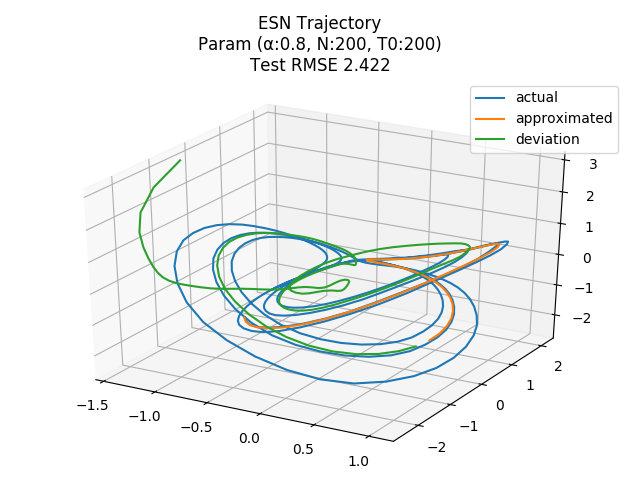
\includegraphics[width=\textwidth]{doc/paper/images/lorenz/rank_0_param_225_fit.png}
        \caption{The True Figure vs ESN Prediction}
        \label{fig:lorenz_r0_fit}
    \end{subfigure}
    ~
    \begin{subfigure}[b]{0.45\textwidth}
        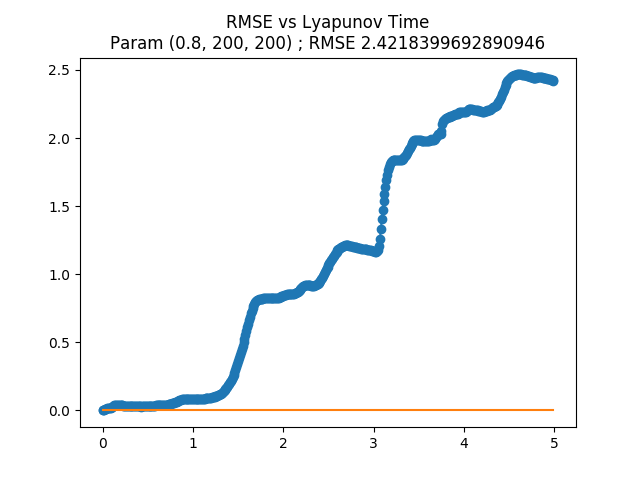
\includegraphics[width=\textwidth]{doc/paper/images/lorenz/rank_0_param_225_rmse.png}
        \caption{RMSE Over Time}
        \label{fig:lorenz_r0_rmse}
    \end{subfigure}
    \caption{The model diverges when entering never seen region.}
    \label{fig:lorenz_r0}
\end{figure}

\begin{figure}[H]
    \centering
    \begin{subfigure}[b]{0.45\textwidth}
        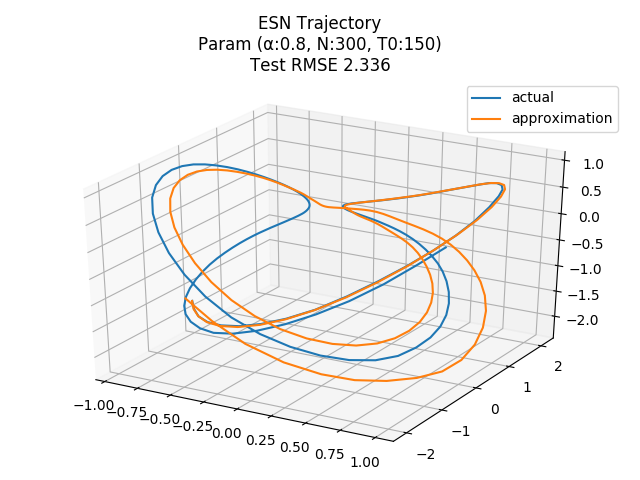
\includegraphics[width=\textwidth]{doc/paper/images/lorenz/rank_1_param_230_fit.png}
        \caption{The True Figure vs ESN Prediction}
        \label{fig:lorenz_r1_fit}
    \end{subfigure}
    ~
    \begin{subfigure}[b]{0.45\textwidth}
        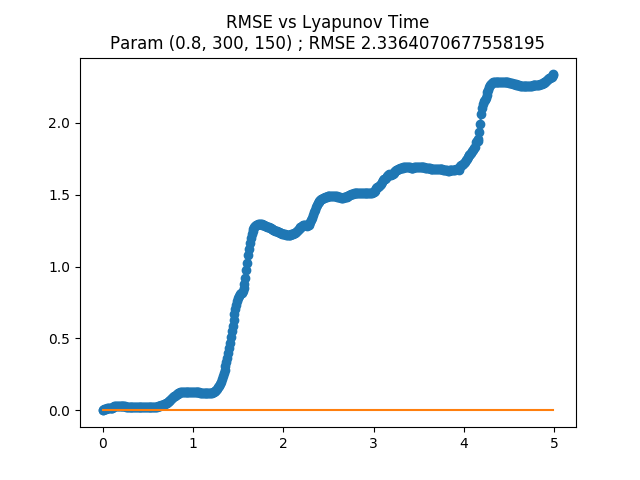
\includegraphics[width=\textwidth]{doc/paper/images/lorenz/rank_1_param_230_rmse.png}
        \caption{RMSE Over Time}
        \label{fig:lorenz_r1_rmse}
    \end{subfigure}
    \caption{The model continues in wrong direction after intersection.}
    \label{fig:lorenz_r1}
\end{figure}

\begin{figure}[H]
    \centering
    \begin{subfigure}[b]{0.45\textwidth}
        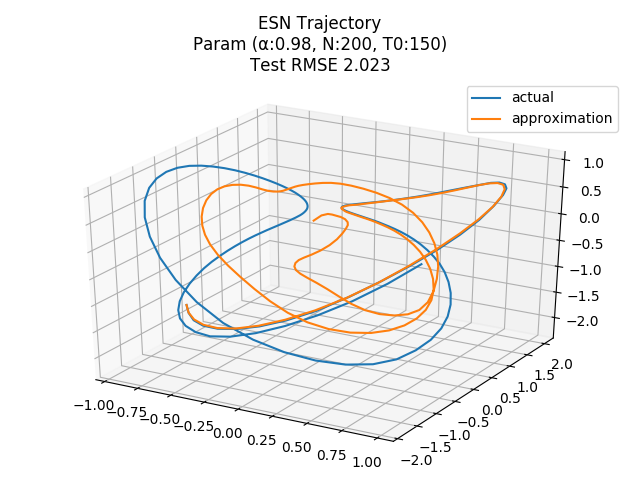
\includegraphics[width=\textwidth]{doc/paper/images/lorenz/rank_2_param_458_fit.png}
        \caption{The True Figure vs ESN Prediction}
        \label{fig:lorenz_r2_fit}
    \end{subfigure}
    ~
    \begin{subfigure}[b]{0.45\textwidth}
        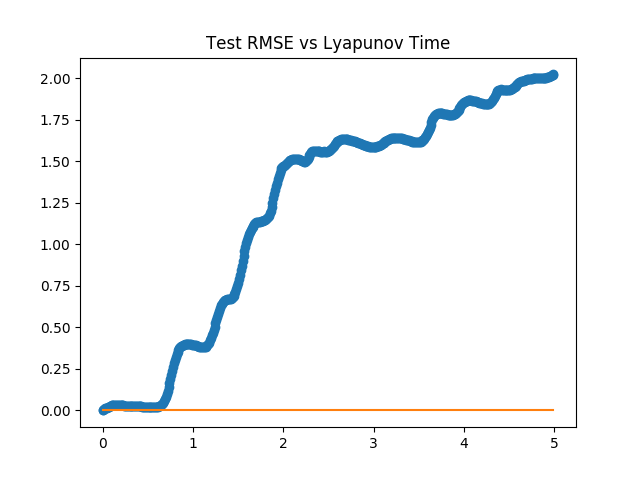
\includegraphics[width=\textwidth]{doc/paper/images/lorenz/rank_2_param_458_rmse.png}
        \caption{RMSE Over Time}
        \label{fig:lorenz_r2_rmse}
    \end{subfigure}
    \caption{The model has completely deviated after an intersection.}
    \label{fig:lorenz_r2}
\end{figure}

\begin{figure}[H]
    \centering
    \begin{subfigure}[b]{0.45\textwidth}
        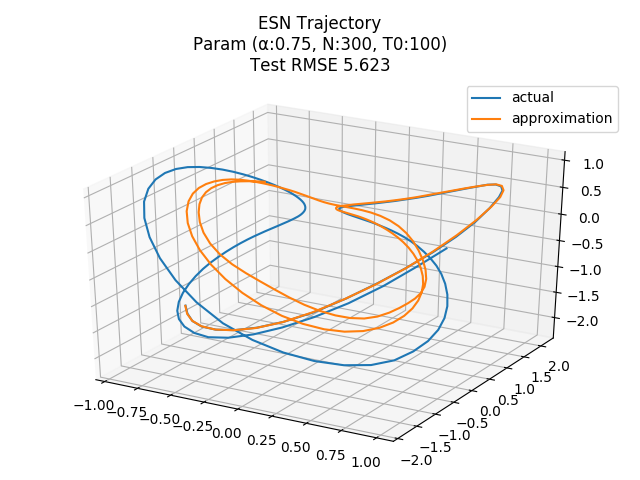
\includegraphics[width=\textwidth]{doc/paper/images/lorenz/rank_3_param_151_fit.png}
        \caption{The True Figure vs ESN Prediction}
        \label{fig:lorenz_r3_fit}
    \end{subfigure}
    ~
    \begin{subfigure}[b]{0.45\textwidth}
        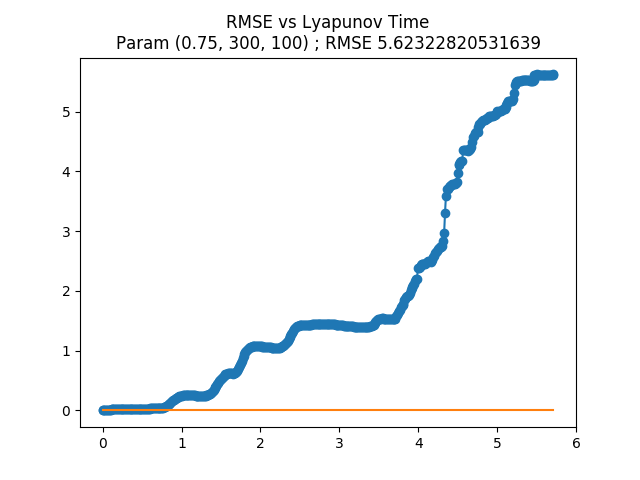
\includegraphics[width=\textwidth]{doc/paper/images/lorenz/rank_3_param_151_rmse.png}
        \caption{RMSE Over Time}
        \label{fig:lorenz_r3_rmse}
    \end{subfigure}
    \caption{Fits model really well, but follows wrong wings.}
    \label{fig:lorenz_r3}
\end{figure}

\begin{figure}[H]
    \centering
    \begin{subfigure}[b]{0.45\textwidth}
        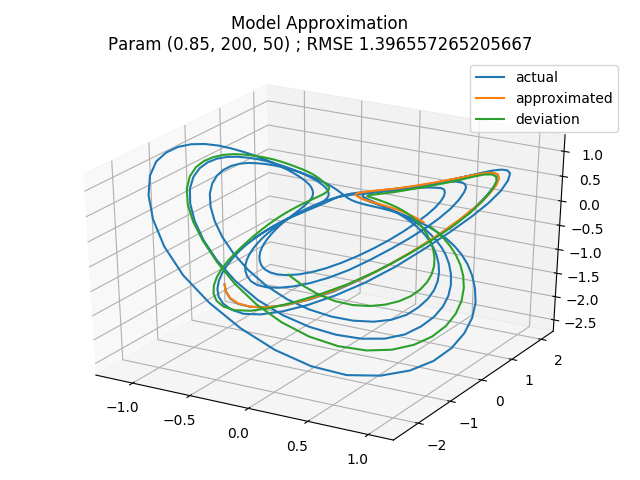
\includegraphics[width=\textwidth]{doc/paper/images/lorenz/rank_4_param_300_fit.png}
        \caption{The True Figure vs ESN Prediction}
        \label{fig:lorenz_r4_fit}
    \end{subfigure}
    ~
    \begin{subfigure}[b]{0.45\textwidth}
        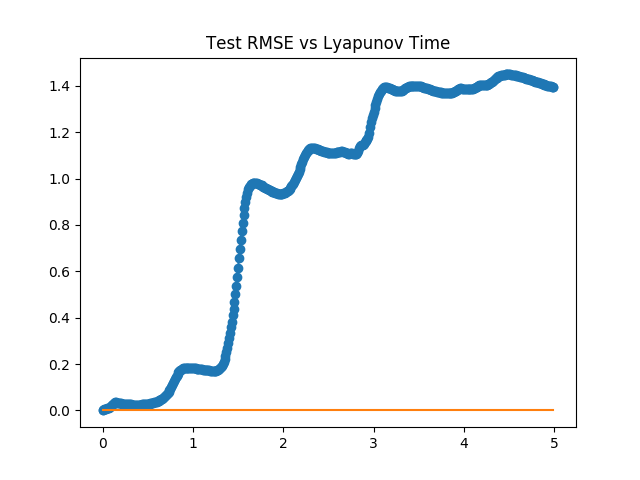
\includegraphics[width=\textwidth]{doc/paper/images/lorenz/rank_4_param_300_rmse.png}
        \caption{RMSE Over Time}
        \label{fig:lorenz_r4_rmse}
    \end{subfigure}
    \caption{Fits model really well, but follows wrong wings.}
    \label{fig:lorenz_r4}
\end{figure}

\begin{figure}[H]
    \centering
    \begin{subfigure}[b]{0.45\textwidth}
        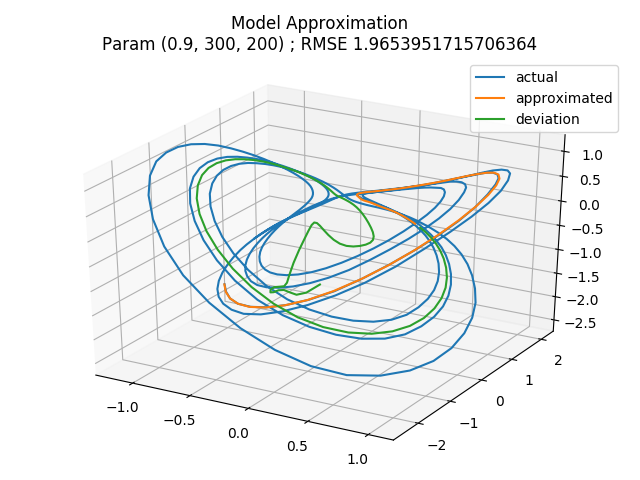
\includegraphics[width=\textwidth]{doc/paper/images/lorenz/rank_5_param_387_fit.png}
        \caption{The True Figure vs ESN Prediction}
        \label{fig:lorenz_r5_fit}
    \end{subfigure}
    ~
    \begin{subfigure}[b]{0.45\textwidth}
        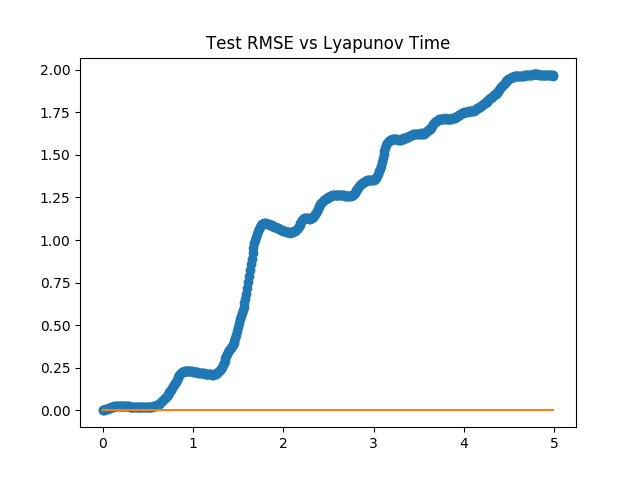
\includegraphics[width=\textwidth]{doc/paper/images/lorenz/rank_5_param_387_rmse.png}
        \caption{RMSE Over Time}
        \label{fig:lorenz_r5_rmse}
    \end{subfigure}
    \caption{Diverges after reaching unknown space.}
    \label{fig:lorenz_r5}
\end{figure}

\begin{figure}[H]
    \centering
    \begin{subfigure}[b]{0.45\textwidth}
        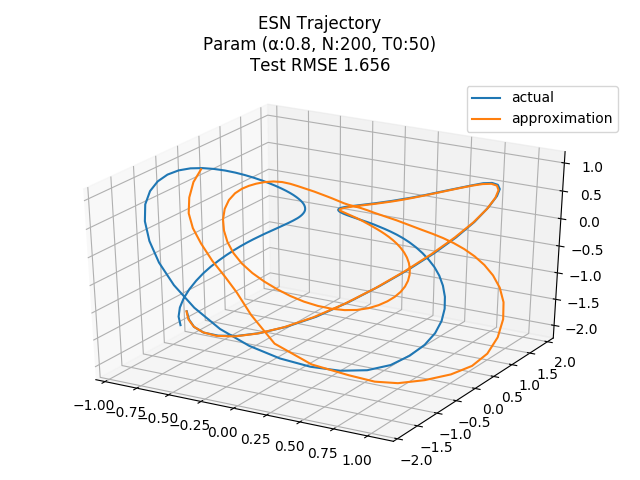
\includegraphics[width=\textwidth]{doc/paper/images/lorenz/rank_6_param_222_fit.png}
        \caption{The True Figure vs ESN Prediction}
        \label{fig:lorenz_r6_fit}
    \end{subfigure}
    ~
    \begin{subfigure}[b]{0.45\textwidth}
        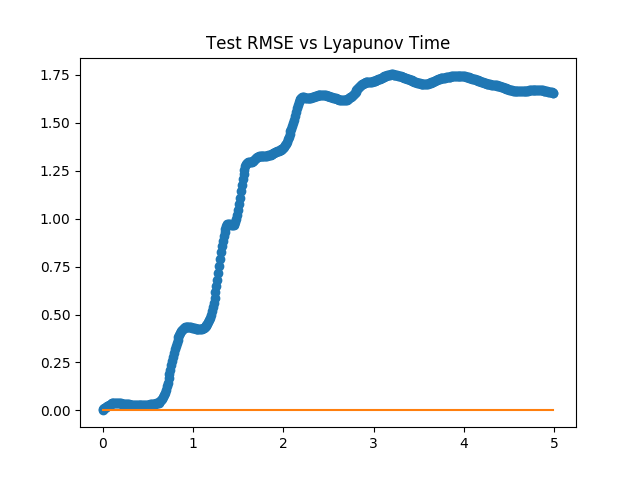
\includegraphics[width=\textwidth]{doc/paper/images/lorenz/rank_6_param_222_rmse.png}
        \caption{RMSE Over Time}
        \label{fig:lorenz_r6_rmse}
    \end{subfigure}
    \caption{Doesn't fit model smoothy and eventually diverges.}
    \label{fig:lorenz_r6}
\end{figure}

\begin{figure}[H]
    \centering
    \begin{subfigure}[b]{0.45\textwidth}
        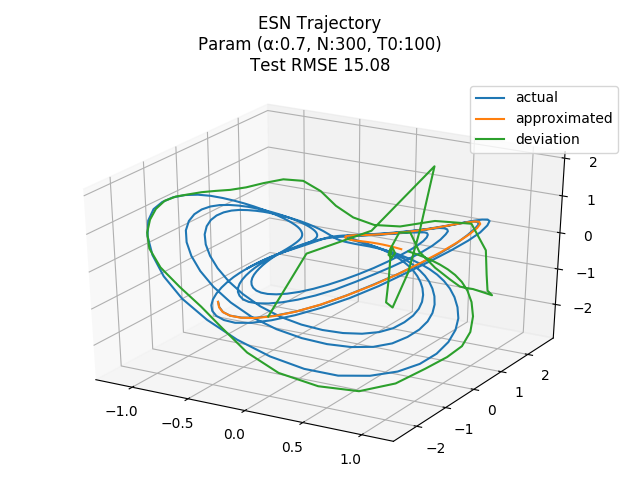
\includegraphics[width=\textwidth]{doc/paper/images/lorenz/rank_7_param_73_fit.png}
        \caption{The True Figure vs ESN Prediction}
        \label{fig:lorenz_r7_fit}
    \end{subfigure}
    ~
    \begin{subfigure}[b]{0.45\textwidth}
        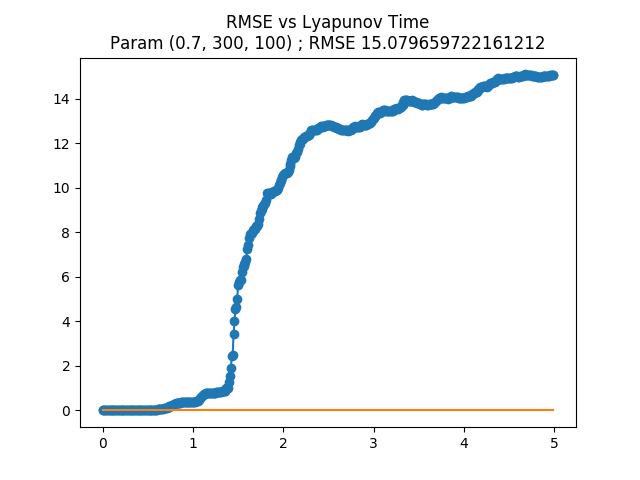
\includegraphics[width=\textwidth]{doc/paper/images/lorenz/rank_7_param_73_rmse.png}
        \caption{RMSE Over Time}
        \label{fig:lorenz_r7_rmse}
    \end{subfigure}
    \caption{Sporadic behavior shown long after divergence.}
    \label{fig:lorenz_r7}
\end{figure}

\subsubsection{Double Pendulum}

The double pendulum's initial condition was

\begin{equation}
(\theta_1, \theta_2, \omega_1, \omega_2) 
= (4.66648088, 4.29820501,
8.01585663 \times 10^{-4}, 3.71175422 \times 10^{-3}).
\end{equation}

In this case, we need $\theta_1$ large enough that the system is chaotic, but
the rest of the parameters were chosen randomly (with rotational velocities
close to zero). The resulting Lyapunov Exponent is $0.60074$. Like the
Lorenz, the differences between time points were used to train the ESN since
the ESN was showing poor results otherwise. As the pendulum kept looping the
center, $\theta_1$ and $\theta_2$ kept growing; this shouldn't be an issue,
but using the differences keeps the system variables in a closer range.

Figure \ref{fig:doub_pend_diff} shows a plot of each of the dataset's
dimensions. It seems like the dataset's activity is fairly sparse. There is
only gradual but seemingly random variations until a few spots around $t=10,
30, 60, \text{and} 75$. The results for the ESN weren't very strong, but it
was able to predict almost two Lyapunov Times before diverging.

Because there are portions of the dataset which are calm, the ESN then has to
pickup on signals which lead to the spikes in movement. We see the testing
graph that while it predicts the testing set well, it eventually tries to
predict spikes but does so at the wrong time, and the spike pattern never
ends, has too large of magnitude, and is very rapid. Overall the model
performs poorly, and it's reflected in the RMSE. The likely reason for this
is that the ESN can't learn the complex patterns from such a small and sparse
dataset.

\begin{figure}[H]
    \centering
    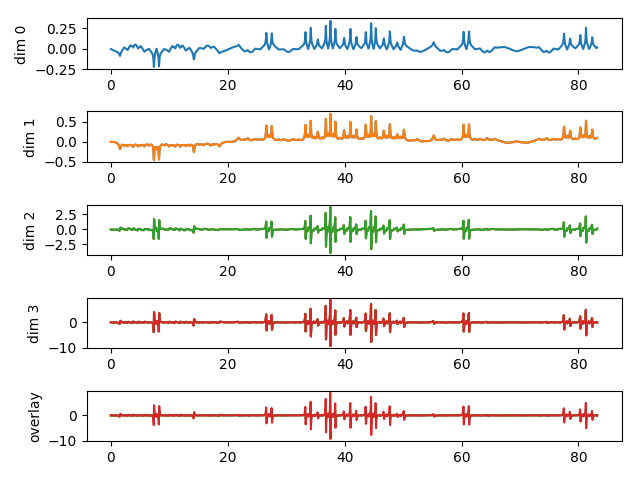
\includegraphics[width=.5\linewidth]{doc/paper/images/doub_pend/full_differential.png}
    \caption{The entire difference dataset}
    \label{fig:doub_pend_diff}
\end{figure}

\begin{figure}[H]
    \centering
    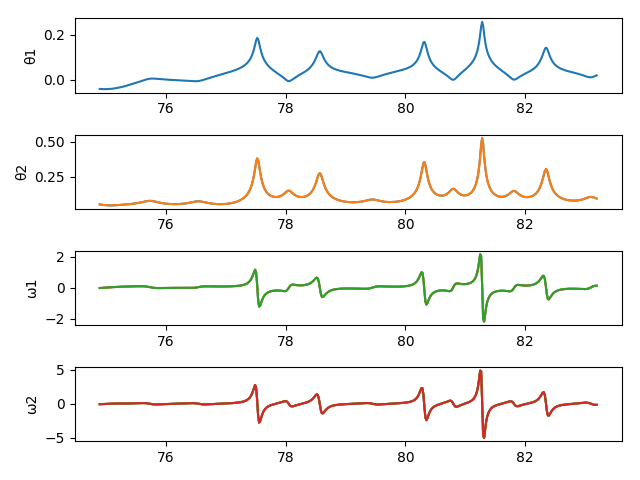
\includegraphics[width=.5\linewidth]{doc/paper/images/doub_pend/test_data.png}
    \caption{The testing dataset partition}
    \label{fig:doub_pend_testing}
\end{figure}

\begin{figure}[H]
    \centering
    \begin{subfigure}[b]{0.45\textwidth}
        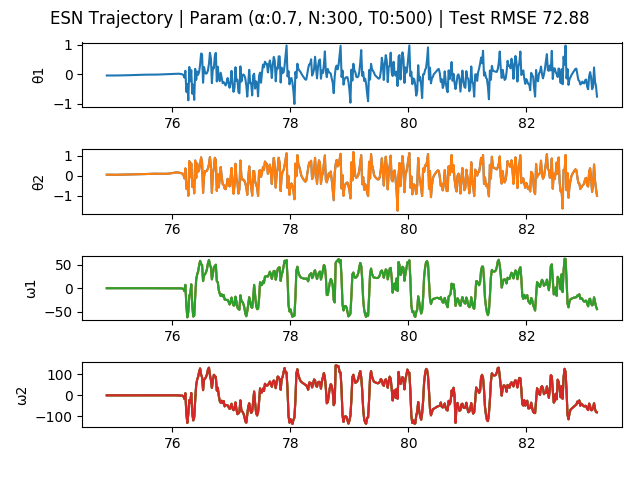
\includegraphics[width=\textwidth]{doc/paper/images/doub_pend/rank_0_param_77_fit.png}
        \caption{Delayed spike prediction}
    \end{subfigure}
    ~
    \begin{subfigure}[b]{0.45\textwidth}
        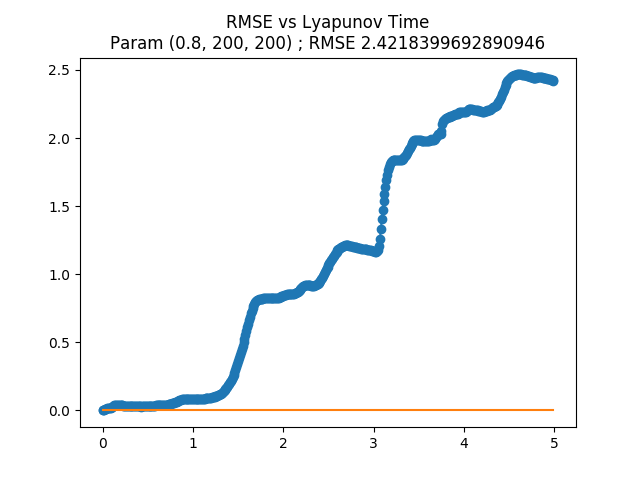
\includegraphics[width=\textwidth]{doc/paper/images/lorenz/rank_0_param_225_rmse.png}
        \caption{RMSE Over Time}
    \end{subfigure}
    \caption{Poor forecast of double pendulum}
\end{figure}

\begin{figure}[H]
    \centering
    \begin{subfigure}[b]{0.45\textwidth}
        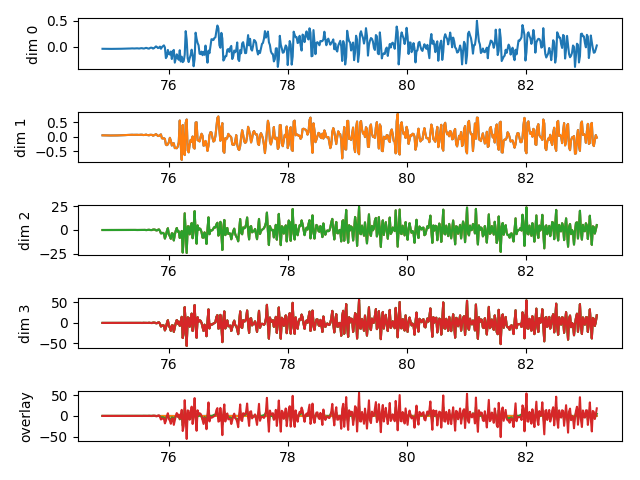
\includegraphics[width=\textwidth]{doc/paper/images/doub_pend/rank_1_param_63_fit.png}
        \caption{Delayed spike prediction}
    \end{subfigure}
    ~
    \begin{subfigure}[b]{0.45\textwidth}
        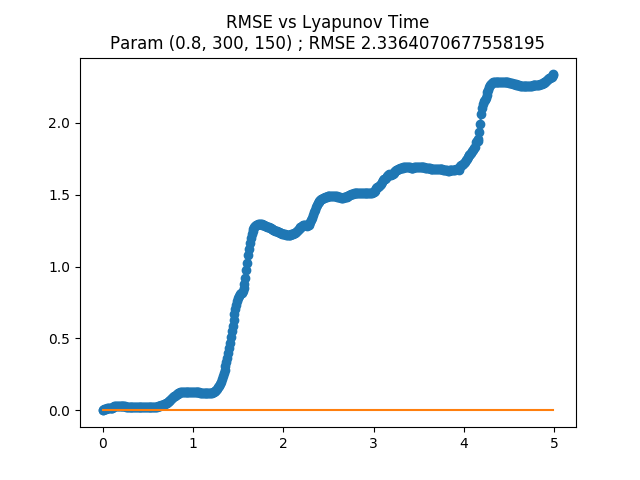
\includegraphics[width=\textwidth]{doc/paper/images/lorenz/rank_1_param_230_rmse.png}
        \caption{RMSE Over Time}
    \end{subfigure}
    \caption{Poor forecast of double pendulum}
\end{figure}

\begin{figure}[H]
    \centering
    \begin{subfigure}[b]{0.45\textwidth}
        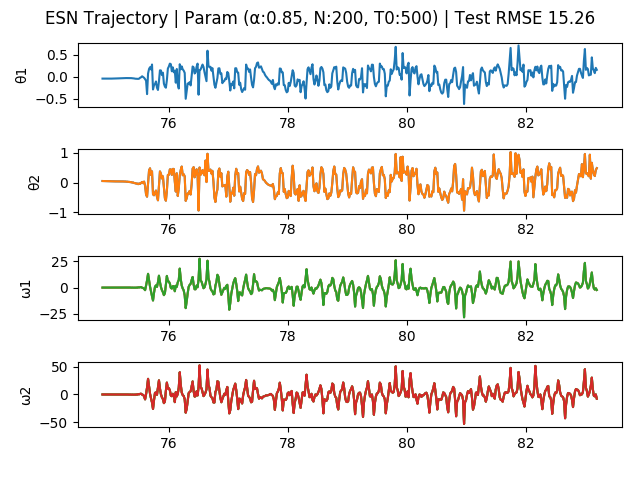
\includegraphics[width=\textwidth]{doc/paper/images/doub_pend/rank_2_param_305_fit.png}
        \caption{Delayed spike prediction}
    \end{subfigure}
    ~
    \begin{subfigure}[b]{0.45\textwidth}
        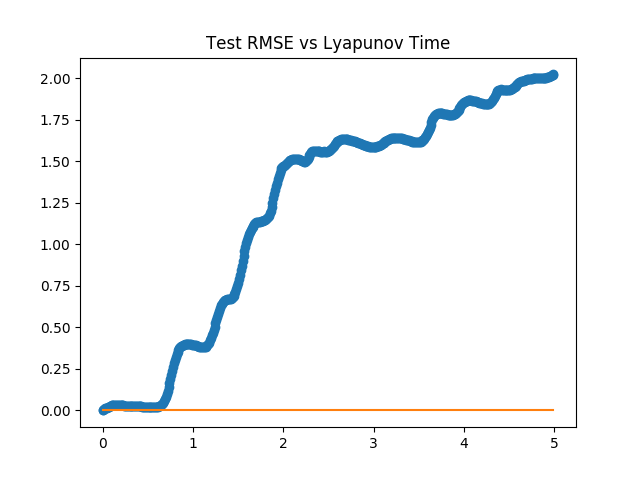
\includegraphics[width=\textwidth]{doc/paper/images/lorenz/rank_2_param_458_rmse.png}
        \caption{RMSE Over Time}
    \end{subfigure}
    \caption{Poor forecast of double pendulum}
\end{figure}

\begin{figure}[H]
    \centering
    \begin{subfigure}[b]{0.45\textwidth}
        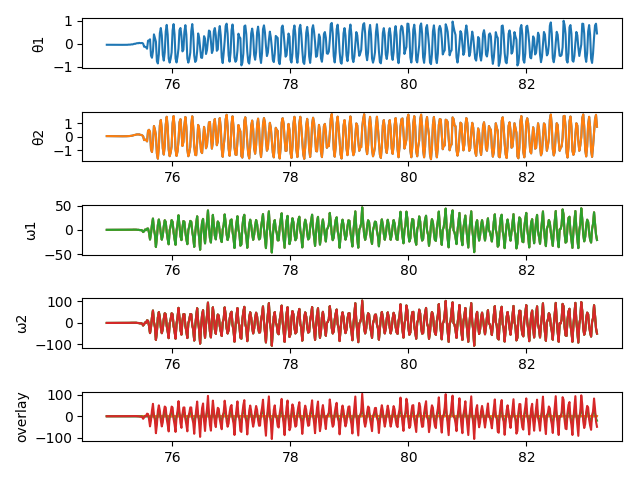
\includegraphics[width=\textwidth]{doc/paper/images/doub_pend/rank_3_param_52_fit.png}
        \caption{Delayed spike prediction}
    \end{subfigure}
    ~
    \begin{subfigure}[b]{0.45\textwidth}
        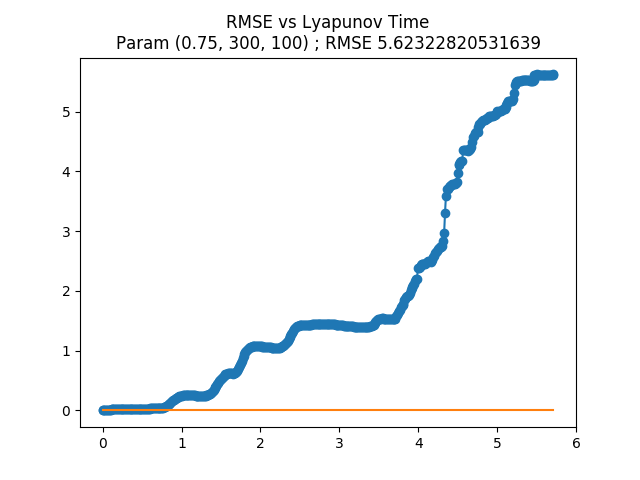
\includegraphics[width=\textwidth]{doc/paper/images/lorenz/rank_3_param_151_rmse.png}
        \caption{RMSE Over Time}
    \end{subfigure}
    \caption{Poor forecast of double pendulum}
\end{figure}

\begin{figure}[H]
    \centering
    \begin{subfigure}[b]{0.45\textwidth}
        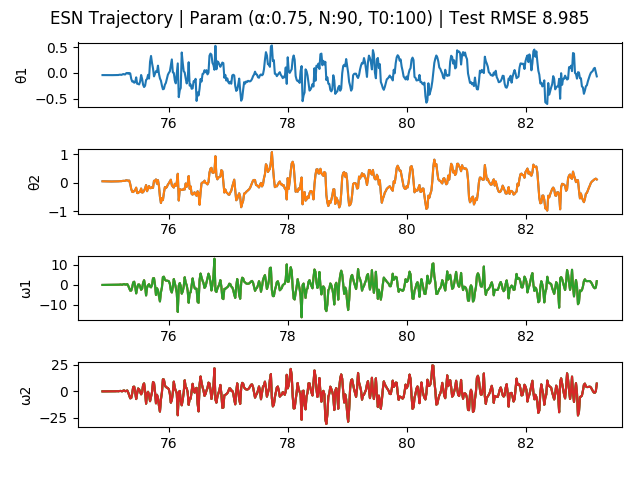
\includegraphics[width=\textwidth]{doc/paper/images/doub_pend/rank_4_param_127_fit.png}
        \caption{Delayed spike prediction}
    \end{subfigure}
    ~
    \begin{subfigure}[b]{0.45\textwidth}
        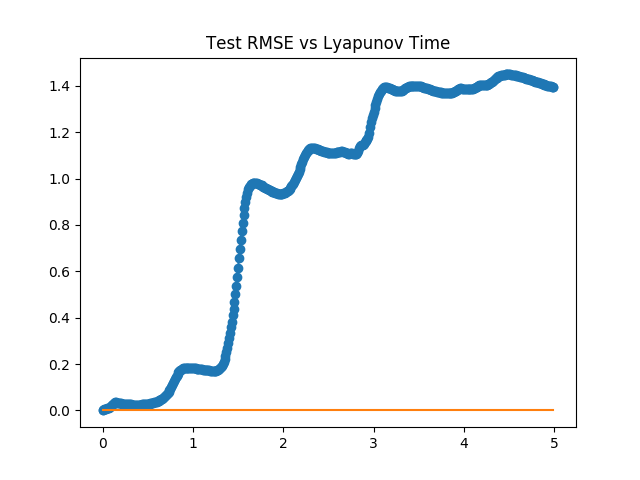
\includegraphics[width=\textwidth]{doc/paper/images/lorenz/rank_4_param_300_rmse.png}
        \caption{RMSE Over Time}
    \end{subfigure}
    \caption{Poor forecast of double pendulum}
\end{figure}

\subsubsection{Restricted Circular 3 Body}

%% CONCLUSION %%%
\section{Conclusion}

\bibliography{references}
\bibliographystyle{unsrt}

\end{document}

% Useful LaTeX commands

%\section{Headings: first level}
%\subsection{Headings: second level}
%\subsubsection{Headings: third level}

%\keywords{First keyword \and Second keyword \and More}

% \paragraph{Paragraph}

%% \begin{figure}
%%   \centering
%%   \fbox{\rule[-.5cm]{4cm}{4cm} \rule[-.5cm]{4cm}{0cm}}
%%   \caption{Sample figure caption.}
%%   \label{fig:fig1}
%% \end{figure}

%%\author{
  %%Lucas Wilson \\
  %%Undergraduate: Mathematics, Computer Science \\
  %%Colorado State University\\
  %%Fort Collins, CO 80523 \\
  %%\texttt{lkwilson96@gmail.com} \\
  %% \AND
  %% Coauthor \\
  %% Affiliation \\
  %% Address \\
  %% \texttt{email} \\
  %% \And
  %% Coauthor \\
  %% Affiliation \\
  %% Address \\
  %% \texttt{email} \\
  %% \And
  %% Coauthor \\
  %% Affiliation \\
  %% Address \\
  %% \texttt{email} \\
%%}
